%%%%%%%% ICML 2021 EXAMPLE LATEX SUBMISSION FILE %%%%%%%%%%%%%%%%%

\documentclass{article}

% Recommended, but optional, packages for figures and better typesetting:
\usepackage{microtype}
\usepackage{graphicx}
\usepackage{subfigure}
\usepackage{booktabs}   % for professional tables
\usepackage{multirow}
\usepackage{amsmath}

% hyperref makes hyperlinks in the resulting PDF.
\usepackage{hyperref}

% Attempt to make hyperref and algorithmic work together better:
\newcommand{\theHalgorithm}{\arabic{algorithm}}

% Use the accepted version style
\usepackage[accepted]{icml2021}

\icmltitlerunning{Detecting American Sign Language Using Hand Landmarkers}

\begin{document}

\twocolumn[
\icmltitle{Detecting American Sign Language Using Hand Landmarkers}

\begin{icmlauthorlist}
\icmlauthor{Matthias Van der Elst (852739843)}{ou}
\icmlauthor{Ren\'ee Vroedsteijn (852710952)}{ou}
\end{icmlauthorlist}

\icmlaffiliation{ou}{Open Universiteit}
\icmlcorrespondingauthor{}{}

\icmlkeywords{ASL, Sign Language, Mediapipe, Landmark Detection, Random Forest, Normalization, Machine Learning, KNN, SVM, Logistic Regression}
\vskip 0.3in
]

\section{Introduction}
American Sign Language (ASL) is a visual language primarily used by the deaf and hard of hearing. Automatically recognizing ASL gestures offers numerous societal benefits, including improved accessibility in communication technologies.

This study explores the use of hand landmark detection and machine learning to classify hand gestures from ASL. Using Mediapipe's hand tracking capabilities and a supervised classifier trained on extracted landmarks, we aim to identify which model and normalization techniques yield the highest accuracy.

The central research questions are:
\begin{enumerate}
    \item Which machine learning model achieves the highest classification accuracy on ASL letter recognition?
    \item Which normalization techniques enhance the model's robustness to variations in hand position, size, and lighting?
\end{enumerate}

\section{Methods}
The ASL letter detector consists of two primary components:
(1) a hand landmark detector using Mediapipe's pre-trained
model, and (2) a custom trained model to predict the ASL
letter based on the provided hand landmarks. This section
describes the system architecture and data processing pipeline
in detail.

\subsection{Pipeline Overview}
The data processing pipeline includes:
\begin{itemize}
    \item \textbf{Image Acquisition}: Using a static dataset or webcam capture.
    \item \textbf{Hand Landmark Detection}: Mediapipe detects 21 hand landmarks (x, y, z) per frame or image.
    \item \textbf{Normalization}: Optionally translating the landmarks so the wrist is at the origin and scaling by wrist-to-middle-finger distance (or other strategies).
    \item \textbf{Feature Vectorization}: Flattening the \((x,y,z)\) coordinates into a 63-dimensional vector for each hand.
    \item \textbf{Model Inference}: A machine learning classifier predicts which ASL letter the vector corresponds to.
\end{itemize}

\subsection{Software Architecture}
\textbf{\texttt{load.py}}: Handles data ingestion and preprocessing. It uses Mediapipe to extract landmarks, applies normalization, and returns feature vectors with associated labels. The output is stored in a CSV file for training.

\textbf{\texttt{train\_model.py}}: Imports the CSV, applies a train/test split, and trains various classifiers including \texttt{KNeighborsClassifier}, \texttt{RandomForestClassifier}, \texttt{SVC}, and \texttt{LogisticRegression}. Models are saved using \texttt{joblib}.

\textbf{\texttt{predict\_live.py}}: Performs real-time predictions using OpenCV and Mediapipe. It loads the trained model and applies the same preprocessing steps on live webcam input for instant classification feedback.

\textbf{\texttt{run\_experiments.py}}: Gathers several experiment routines, such as comparing multiple models, testing various normalization strategies, performing dimensionality reduction (PCA/t-SNE) for visualization, and optionally conducting cross-user validation.

\section{Experimental Results}

\subsection{Datasets}
To train the model, a dataset containing 1,728 images of ASL letters under varied conditions was used. This included both colored and grayscale images, with different brightness levels and multiple users. Auto-orientation corrections were applied, and images were resized to 640x640. Approximately 300 images were excluded because the hand landmarks could not be reliably detected (e.g., occlusion or poor lighting).

\subsection{Implementation Details}
\begin{itemize}
    \item \textbf{Data Augmentation}: Horizontal flipping to simulate left/right hands and increase dataset size.
    \item \textbf{Normalization}: Translation of landmarks around the wrist and scaling by the maximum distance (often wrist-to-middle-finger).
    \item \textbf{Train/Test Split}: An 80/20 stratified split.
    \item \textbf{Models Tested}: K-Nearest Neighbors, Random Forest, Support Vector Machine, Logistic Regression.
\end{itemize}

\subsection{Model Comparison Results}
Table \ref{tab:model-comparison} provides a placeholder summary of the four models tested:

\begin{table}[ht]
\centering
\caption{Model Comparison Results (Placeholder)}
\label{tab:model-comparison}
\begin{tabular}{lrrrrr}
\toprule
\textbf{model\_type} & \textbf{accuracy} & \textbf{precision} & \textbf{recall} & \textbf{f1\_score} & \textbf{roc\_auc}\\
\midrule
knn                   & 0.824373 & 0.828397 & 0.811953 & 0.812151 & None \\
random\_forest        & 0.892473 & 0.903509 & 0.887729 & 0.888269 & None \\
svm                   & 0.763441 & 0.775478 & 0.744949 & 0.729576 & None \\
logistic\_regression  & 0.820789 & 0.833100 & 0.811907 & 0.812426 & None \\
\bottomrule
\end{tabular}
\end{table}

\begin{itemize}
    \item \textbf{Highest Accuracy}: Random Forest (0.892).
    \item \textbf{Competitive Models}: KNN and Logistic Regression both near 0.82 accuracy.
    \item \textbf{Lowest Accuracy}: SVM at 0.76.
\end{itemize}

\subsection{Normalization Strategies}
As shown in Table \ref{tab:normalization-results}, these placeholder results indicate that, for the current dataset, different normalization approaches yield similar performance:

\begin{table}[ht]
\centering
\caption{Normalization Strategies Experiment (Placeholder)}
\label{tab:normalization-results}
\begin{tabular}{lrr}
\toprule
\textbf{Strategy} & \textbf{Accuracy} & \textbf{F1-Score} \\
\midrule
none               & 0.89 & 0.89 \\
translation\_only  & 0.89 & 0.89 \\
translation\_scale & 0.89 & 0.89 \\
\bottomrule
\end{tabular}
\end{table}

\textit{Further experiments with rotation correction or alternative scaling references may yield different outcomes.}

\subsection{Dimensionality Reduction and Visualizations}
For 63-dimensional landmark data, PCA and t-SNE offer insights into class separability. Figures \ref{fig:pca-vis} and \ref{fig:tsne-vis} are placeholders:

\begin{figure}[ht]
    \centering
    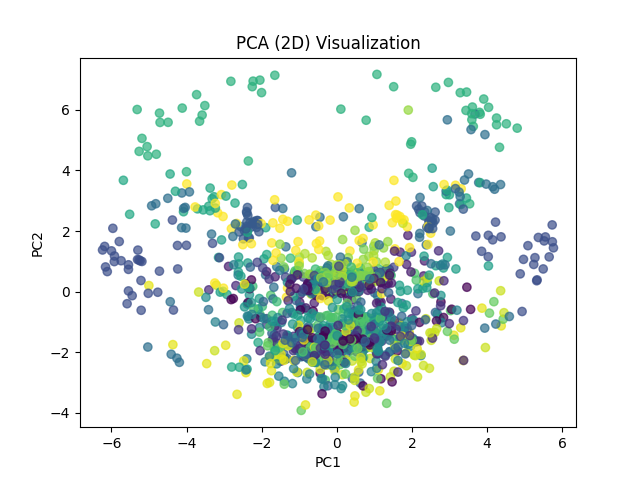
\includegraphics[width=0.8\columnwidth]{pca_visualization.png}
    \caption{PCA Visualization of Hand Landmark Features}
    \label{fig:pca-vis}
\end{figure}

\begin{figure}[ht]
    \centering
    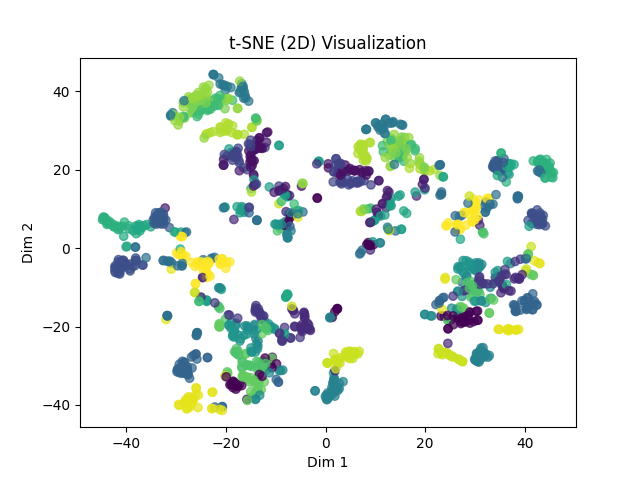
\includegraphics[width=0.8\columnwidth]{tsne_visualization.png}
    \caption{t-SNE Visualization of Hand Landmark Features}
    \label{fig:tsne-vis}
\end{figure}

\subsection{Discussion of Findings}
\textbf{Model Comparison}: Random Forest consistently produced the highest accuracy, suggesting it effectively handles the complex decision boundaries of ASL gestures.

\textbf{Normalization}: Despite different strategies, the models maintained roughly the same performance for this dataset. Future tests might involve more diverse samples or additional normalization steps (like rotation correction).

\textbf{Dimensionality Reduction}: PCA and t-SNE hinted at some class structure, but not perfectly separable in 2D. More specialized features or deeper architectures might help to further distinguish classes.

\section{Conclusion and Future Work}
We demonstrated an ASL recognition pipeline using Mediapipe landmarks and traditional ML classifiers. Random Forest emerged as the top performer, though other models also showed promise. Different normalization methods yielded similar outcomes in these experiments.

Potential directions to explore include:
\begin{itemize}
    \item \textbf{Rotation Correction}: Aligning the hand axis for more robust normalization.
    \item \textbf{Cross-User Validation}: Ensuring the model does not overfit to a single user's hand shape or gestures.
    \item \textbf{Data Augmentation}: Incorporating more challenging conditions such as motion blur or partial occlusion.
    \item \textbf{Live Tests}: Measuring real-time performance and user acceptance across a broader population.
\end{itemize}

\bibliography{references}
\bibliographystyle{icml2021}

\end{document}
